\documentclass [blue] {beamer}
\usepackage{beamerthemesplit}
\usetheme{Boadilla}
%\usecolortheme{orchid}
\setbeamertemplate{footline}[text line]{}
\usepackage [latin1] {inputenc}
\usepackage [T1] {fontenc}
\usepackage{ulem}
\usepackage [french] {babel}
\usepackage {indentfirst}
%\usepackage {graphicx}
\usepackage {geometry}
\usepackage{verbatim}
%% The amssymb package provides various useful mathematical symbols
\usepackage{amssymb}
%% The amsthm package provides extended theorem environments
%\usepackage{amsthm}
\usepackage{amsmath}
\usepackage{enumerate}
\newtheorem{proposition}[theorem]{Proposition}
\usepackage{empheq}
\usepackage{hyperref}
\usepackage{eurosym}
\hypersetup{colorlinks, citecolor=blue,%
filecolor=blue,%
linkcolor=blue,%
urlcolor=blue}
%\setbeamertemplate{blocks}[shadow=false]
\setbeamercovered{transparent}
\defbeamertemplate*{footline}{my theme}
{
\leavevmode
\hbox{
\begin{beamercolorbox}[wd=1\paperwidth,ht=2.25ex,dp=1ex,right,ignorebg]{date in head/foot} \usebeamerfont{date in head/foot}\insertshortdate{}\hspace*{2em}
S�ance 18/ \insertframenumber{} \hspace*{4ex}
\end{beamercolorbox}}%
\vskip0pt%
}
\usepackage{color}
\date{29 avril 2014}
\author{Olivia D'Aoust\\
odaoust@ulb.ac.be}
\title{S�ance 18 \\ Equilibre macro�conomique}
\begin{document}
\frame{\titlepage}
\normalsize

\frame{
\frametitle{Rappel IS-LM}
\begin{center}
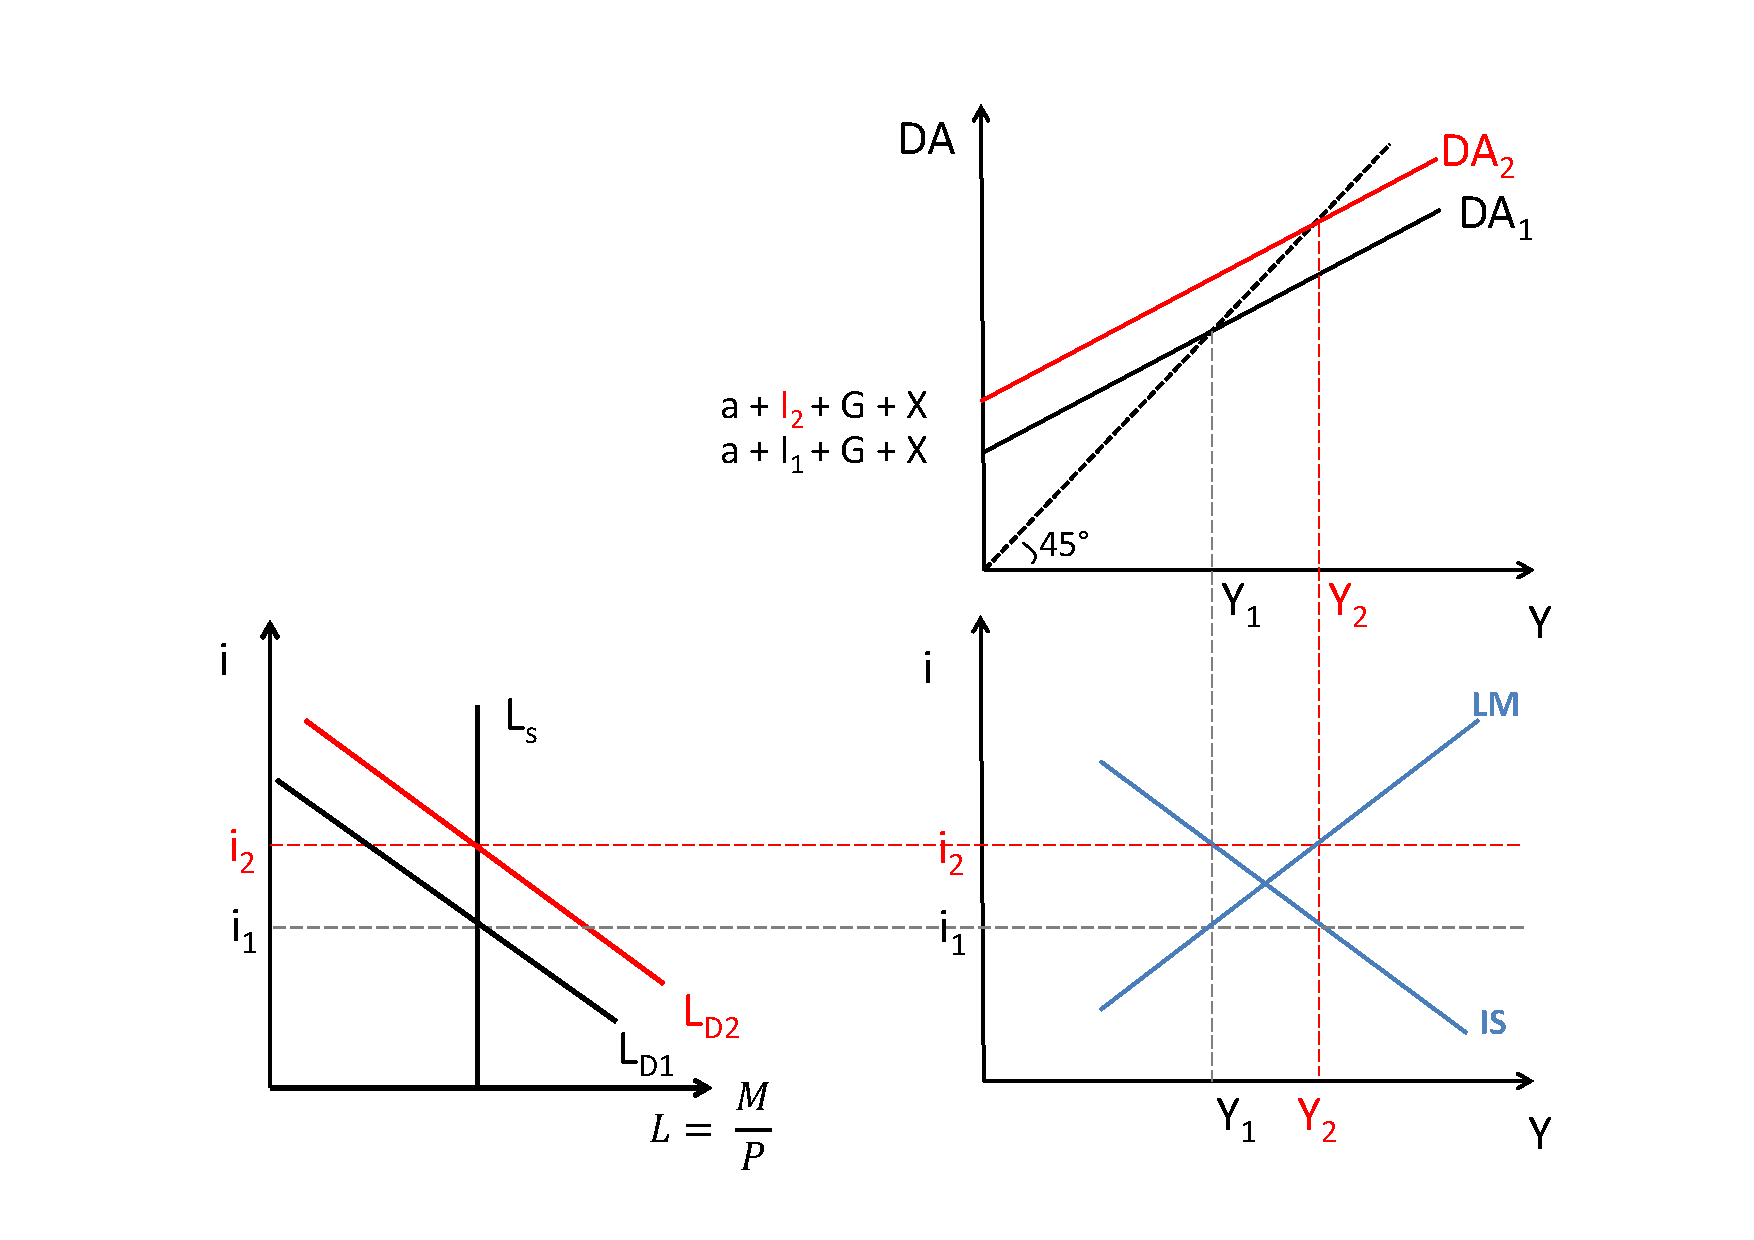
\includegraphics[clip=true, trim = 2cm 0cm 0cm 1cm, scale=0.42]{IS-LM.pdf}
\end{center}


}


\frame{
\frametitle{\large Demande agr�g�e coh�rente avec l'�quilibre mon�taire $Y_d$}

A partir d'IS-LM, on �tablit une relation entre l'output Y et le niveaux des prix P, telle que les march�s sont � l'�quilibre.

\begin{center}
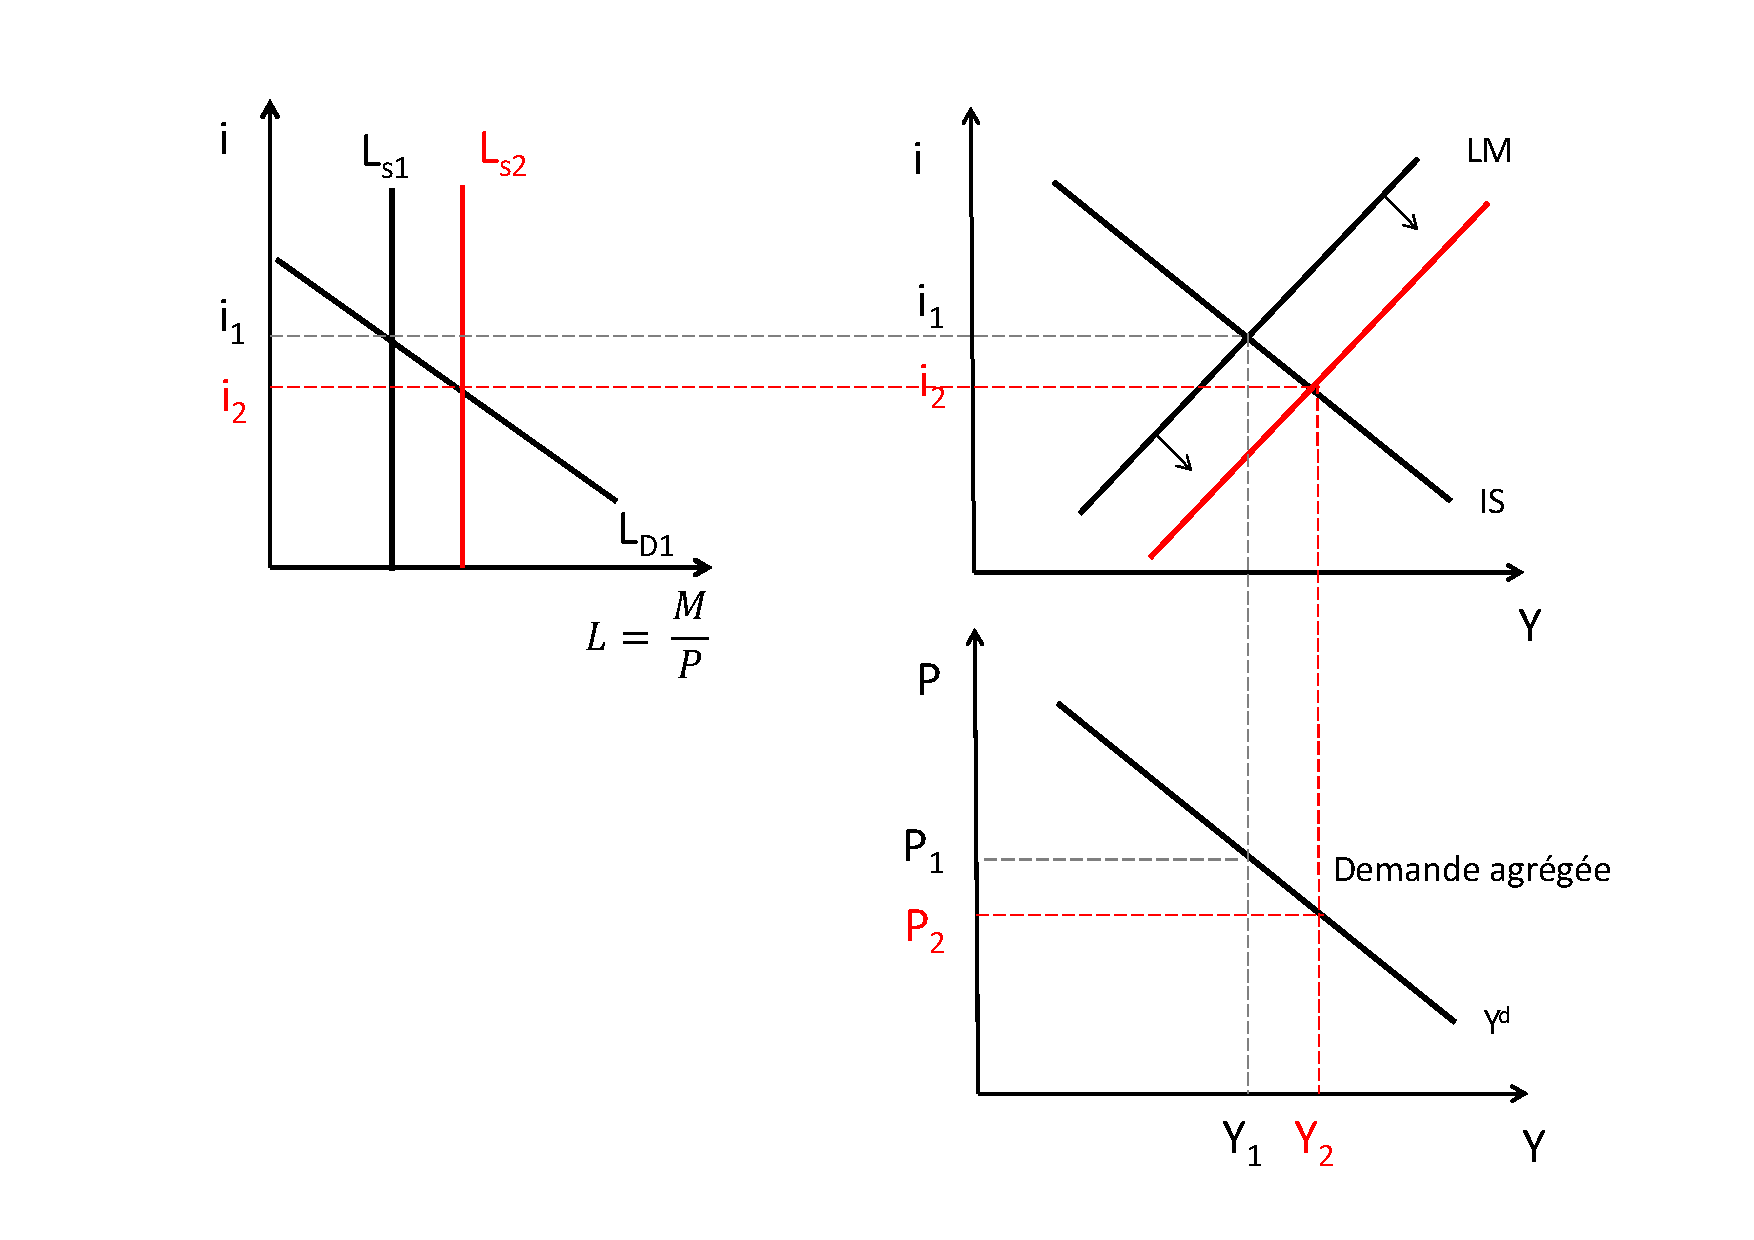
\includegraphics[clip=true, trim = 2cm 0cm 0cm 1cm, scale=0.35]{DA.pdf}
\end{center}


}

\frame{
\frametitle{\large Offre agr�g�e coh�rente avec l'�quilibre sur le march� du travail $Y_s$ }

On ajoute au mod�le l'�quilibre sur le march� du travail afin d'�tablir une relation de long terme entre l'output Y et le niveaux des prix P.

\begin{center}
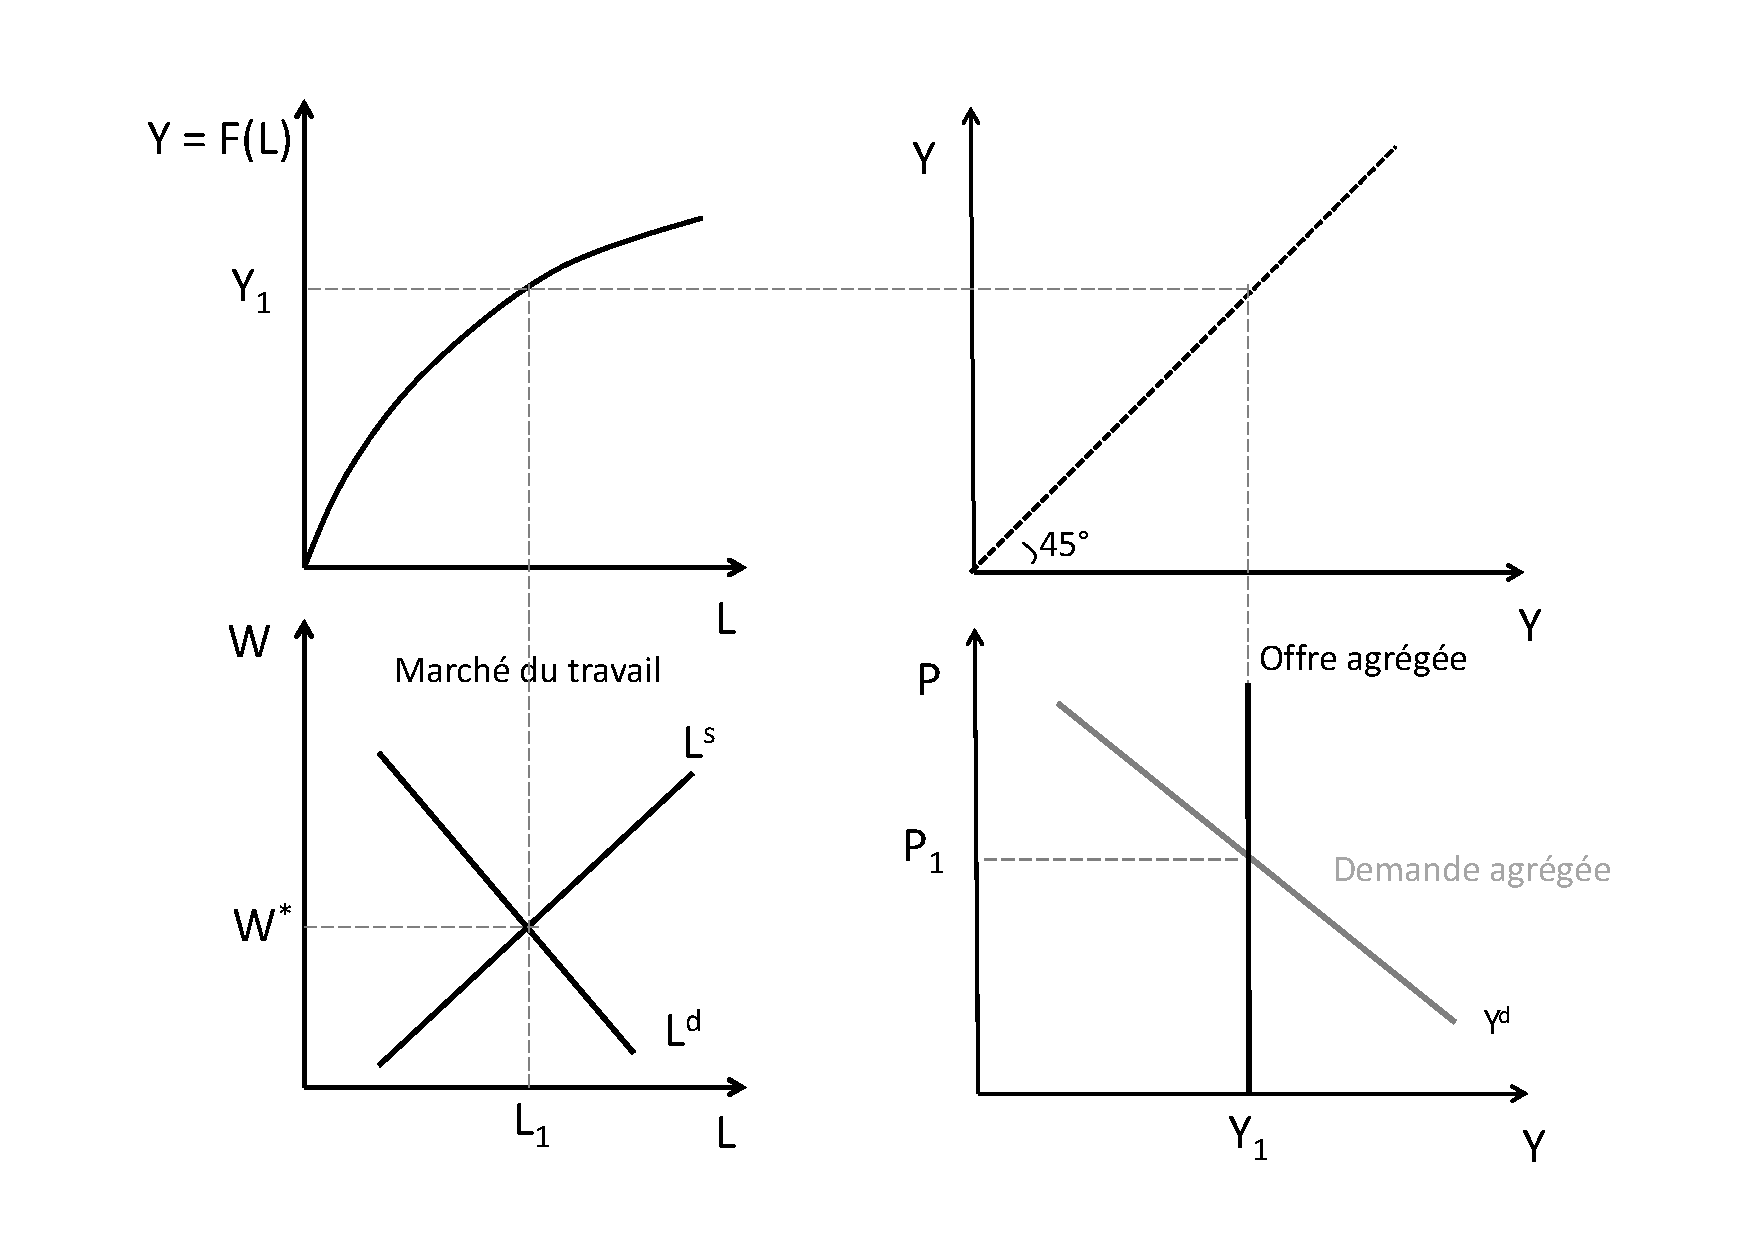
\includegraphics[clip=true, trim = 2cm 0cm 0cm 1cm, scale=0.35]{OA.pdf}
\end{center}

}

\frame{
\frametitle{Equilibre macro�conomique de long terme}

A long terme, l'offre agr�g�e est in�lastique par rapport aux prix. L'�quilibre macro�conomique suppose que le plein emploi (et donc le maximum des capacit�s de production) est atteint sur le march� du travail (qui est � l'�quilibre).

\begin{center}
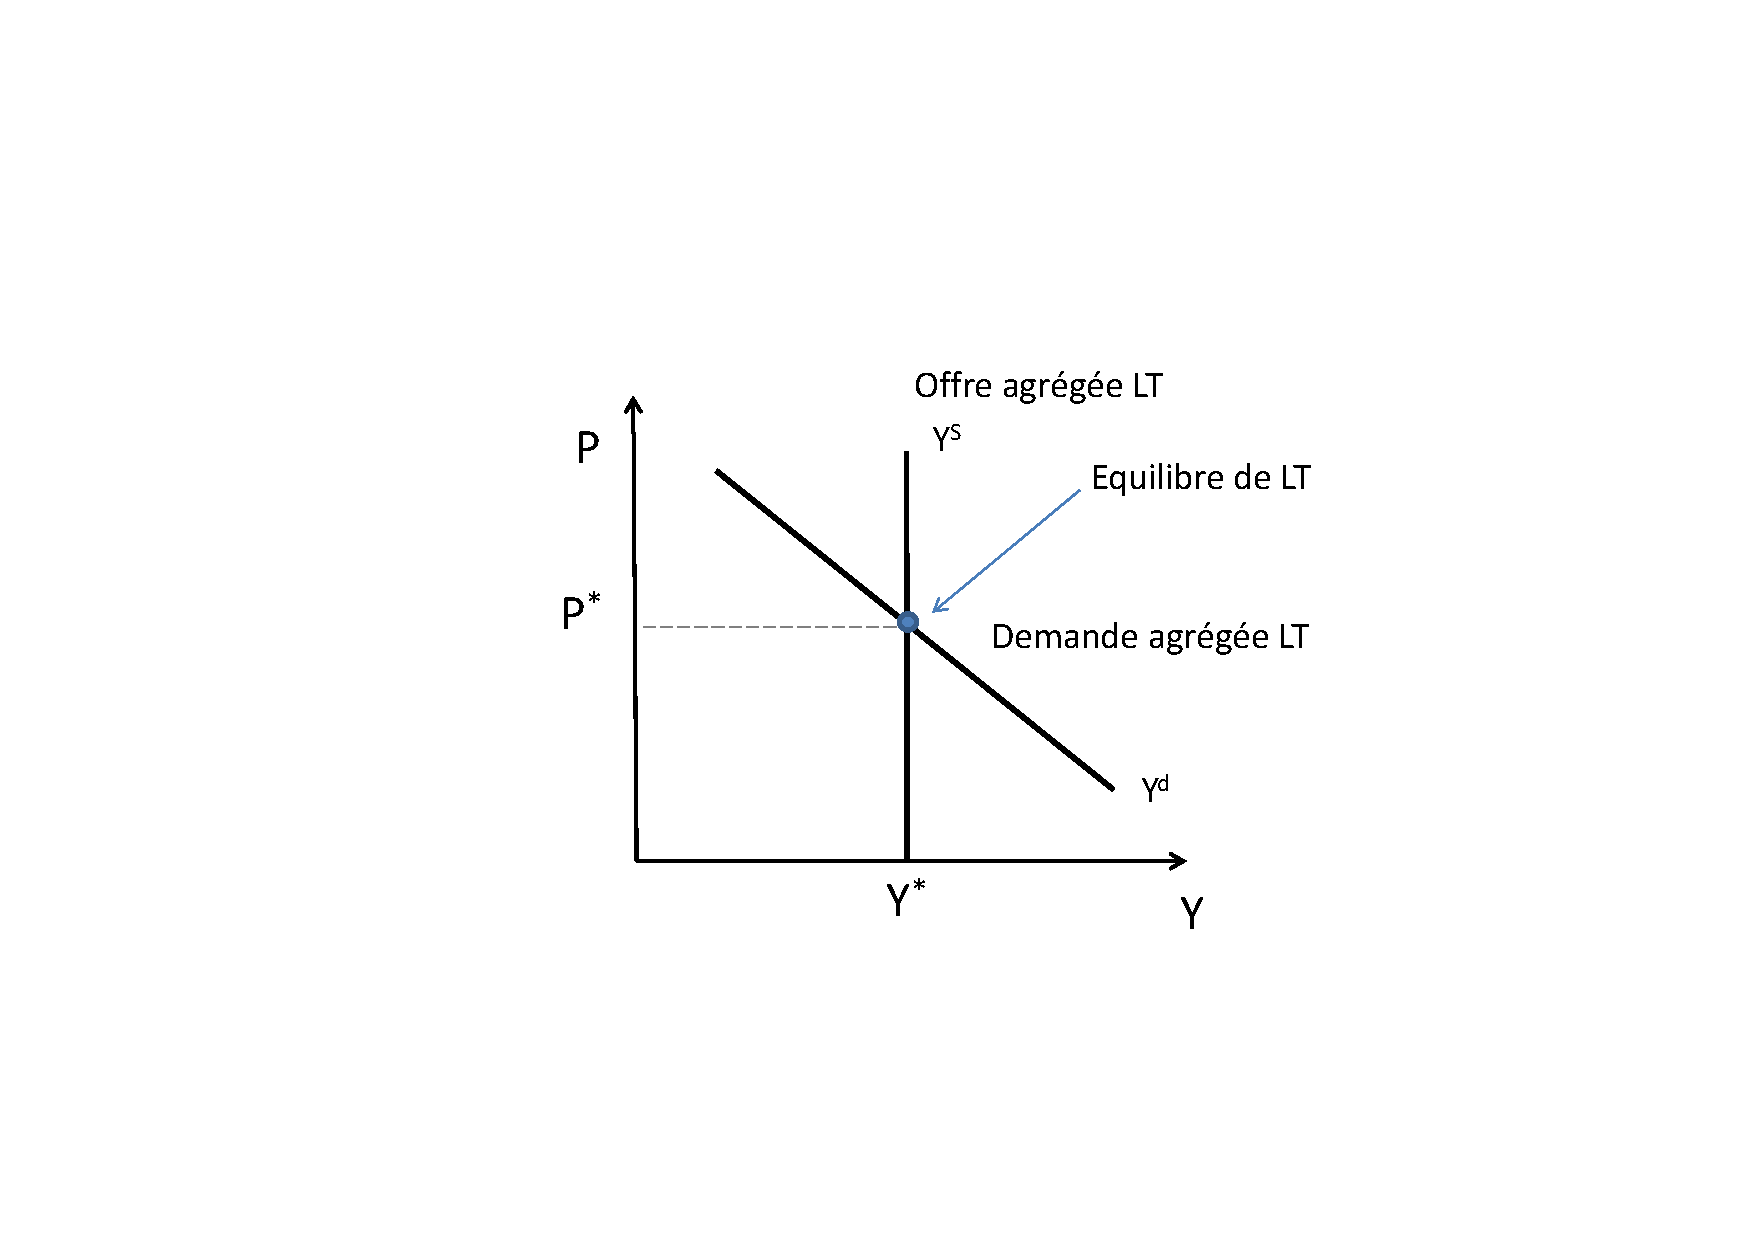
\includegraphics[clip=true, trim = 5cm 5cm 5cm 5.4cm, scale=0.6]{eq.pdf}
\end{center}

}

\frame{
\frametitle{A court terme}
\small
L'offre de travail peut �tre diff�rente de celle du plein emploi en raison de ...\\[0.08cm]

1) \textbf{la rigidit� des salaires ($Y^{CT}_s < Y^{LT}_s$)}\\
\it{\footnotesize{Suite � une \emph{baisse} des prix (et une hausse de $w_r$), le salaire nominal est rigide � la baisse. Il y a un exc�s d'offre de travail sur ce march�.}}
\begin{center}
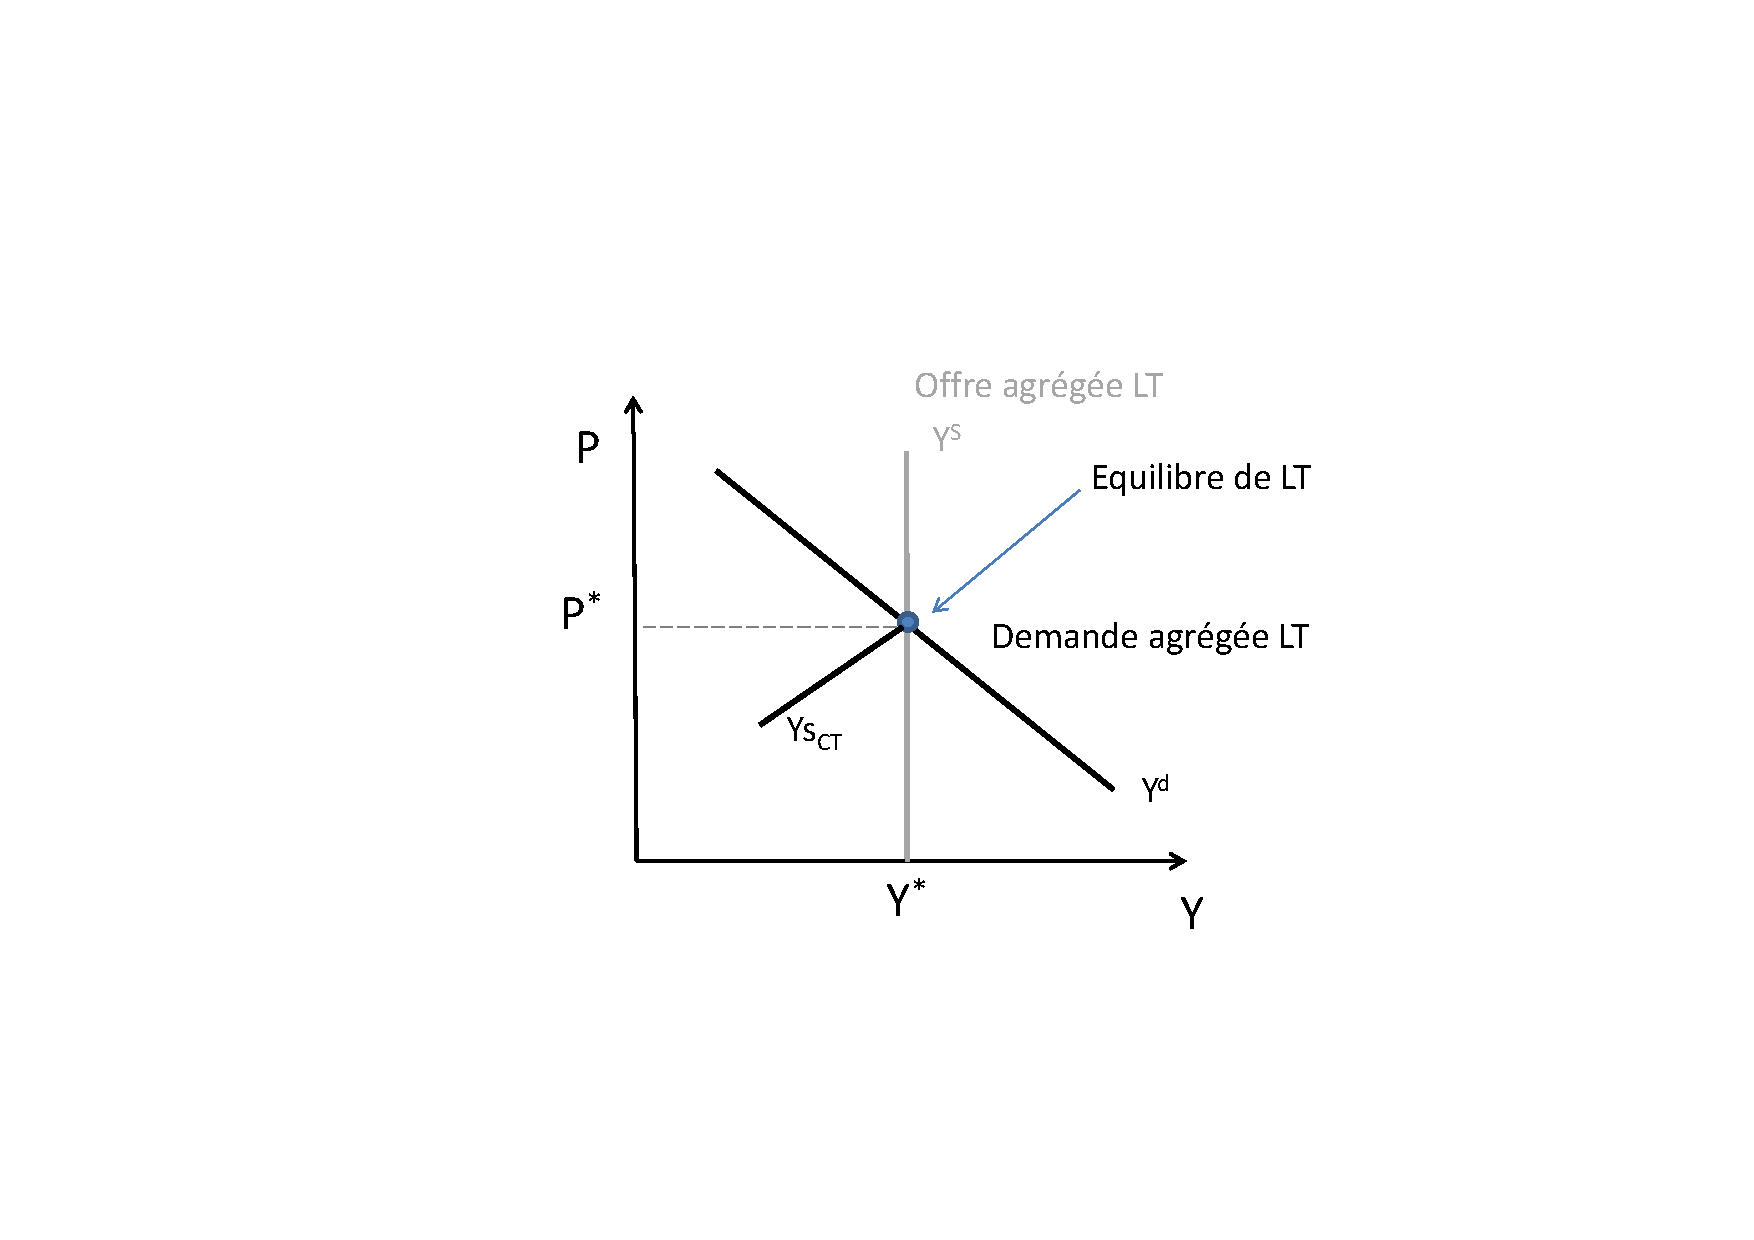
\includegraphics[clip=true, trim = 5cm 5cm 5cm 5cm, scale=0.6]{ysCT.pdf}
\end{center}

}

\frame{
\frametitle{A court terme}
\small
L'offre de travail peut �tre diff�rente de celle du plein emploi en raison de ...\\[0.08cm]

2) \textbf{l'illusion mon�taire ($Y^{CT}_s > Y^{LT}_s$)}\\
\it{\footnotesize{Suite � une \emph{hausse} des prix (et une baisse de $w_r$), les agents ne s'adaptent pas et maintiennent leur offre d'emploi}}
\begin{center}
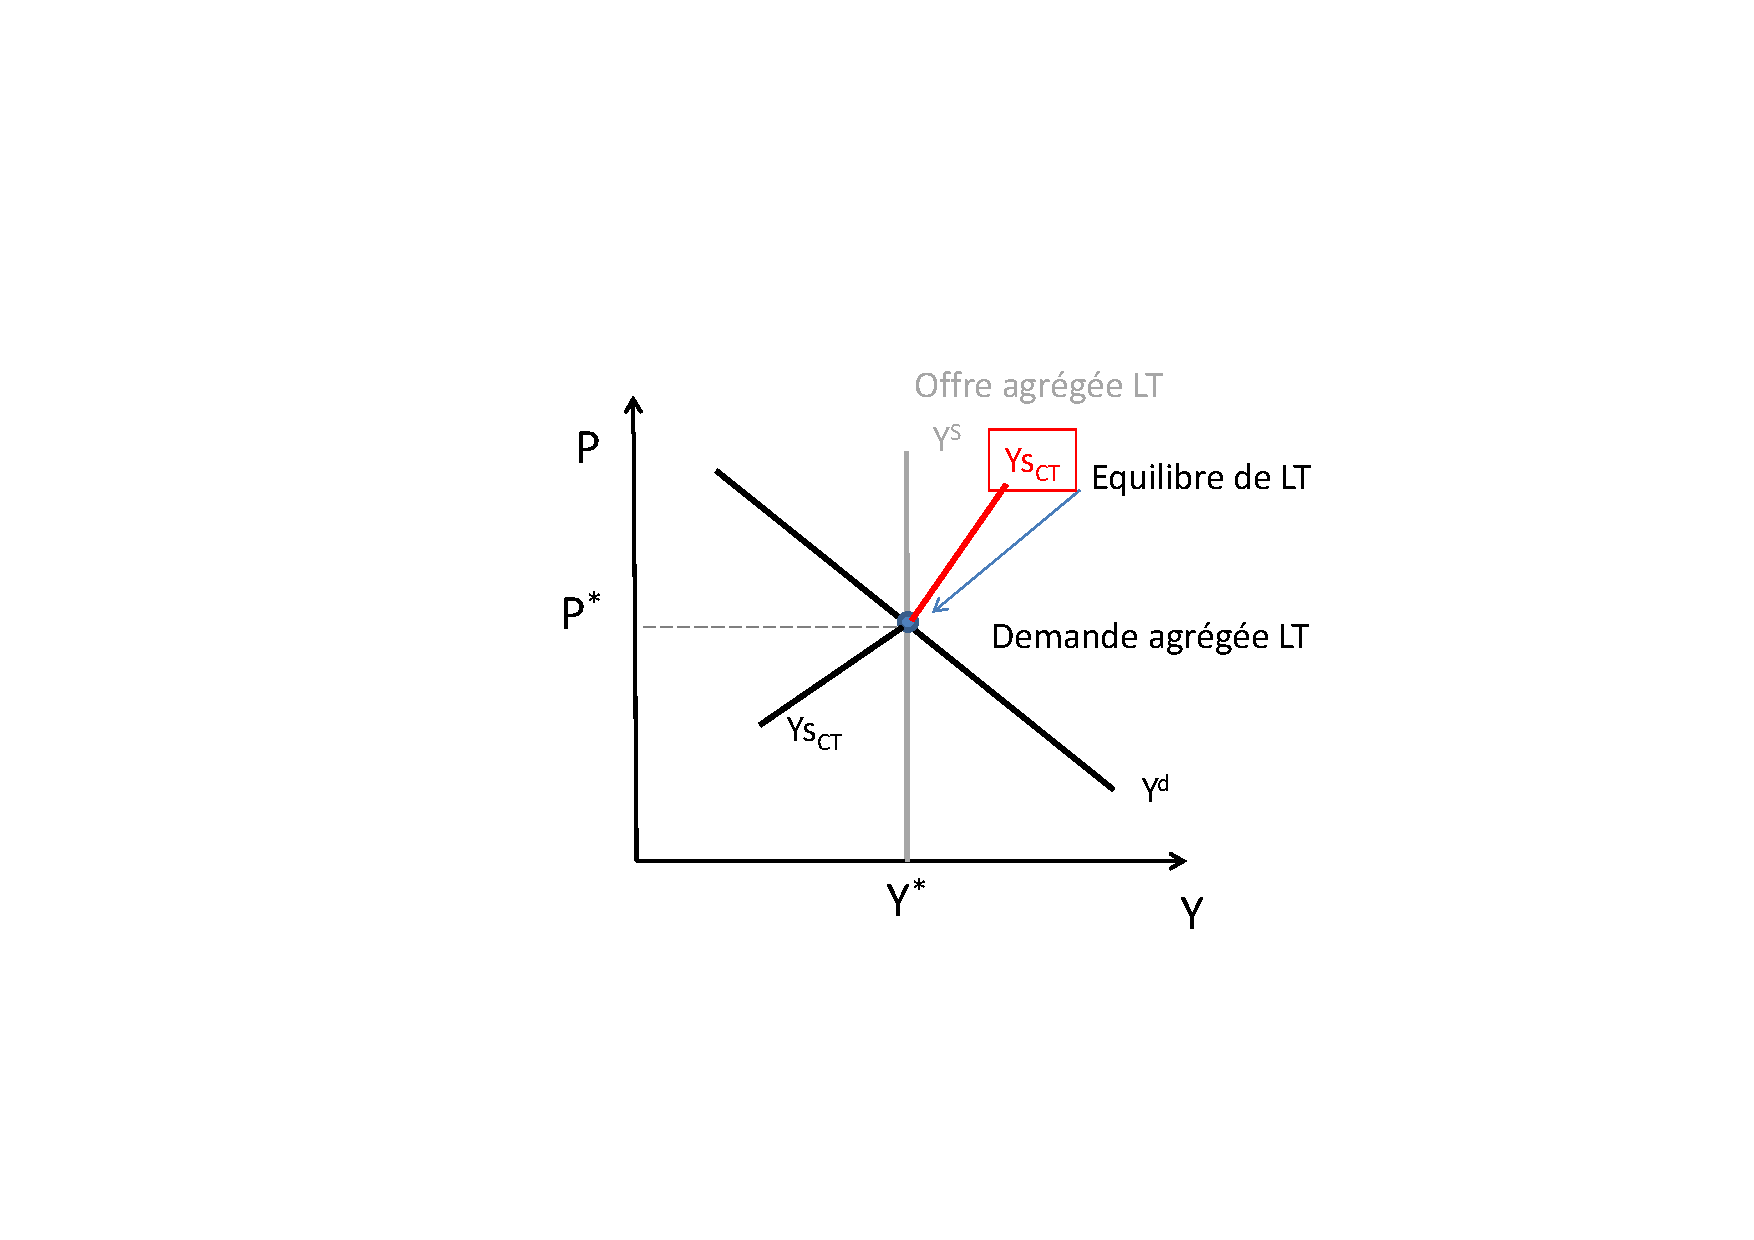
\includegraphics[clip=true, trim = 5cm 5cm 5cm 5cm, scale=0.6]{ysLT.pdf}
\end{center}

}


\frame{
\frametitle{Exercices suppl�mentaires}
\footnotesize
\textbf{Exercice 6}\\
a) F\\
b) I\\
c) G\\
d) L\\
e) A\\
f) C\\[0.3cm]

\textbf{Exercice 7}\\

a) situation initiale en $y_4, i_3$ \\
b) Apr�s $\Delta^+$P, en absence d'effet d'encaisses r�elles: on est en $y_3, i_4, P_2$\\
c) Apr�s $\Delta^+$P, en pr�sence d'effet d'encaisses r�elles: on est en $y_1, i_2, P_2$\\[0.3cm]

\textbf{Exercice 8}\\
Les propositions a) et c) sont correctes. \\
e) 2\\
f) 3\\
g) 6\\[0.3cm]

\textbf{Exercice 9}\\
Les propositions a), b), c), d), e), g), h), m), p) et r) sont correctes \\[0.3cm]
}


\end{document}
